%!TEX root = report.tex
\section{Grafisk fremstilling}\label{sec:artwork}
Under vil den grafiske fremstillingen av \emph{Garbage Alert} bli beskrevet
sammen med valgene som har blitt gjort. Dette vil illustreres med
skjermskudd.

Den grafiske fremstillingen i spillet er ment å være leken og rettet mot
barn i alle aldre, og er sterkt inspirert av den klassiske spillserien
Advance Wars (se appendiks \ref{app:aw}). Videre har det å holde ting oversiktlig og stort nok til å
trykkes på en berøringsskjerm vært noe vi har hatt spesielt i tankene
når grensesnittet har blitt utformet. Det er lagt mer vekt på
funksjonalitet, enn selve fremstillingen på denne delen av stadiet. Av
skjermskuddene ser en to forskjellige spillere som spiller mot
hverandre.

Som en ser av figur~\ref{fig:Oppgradering} kan spilleren på dette
tidspunktet kun oppgradere til plast. Dette er med andre ord i en tidlig
fase av spillet. Tilgjengelige ressurser er vist i bunnen av
skjermskuddet, og på dette tidspunktet kan miljøstasjonen kun gjenvinne
plast.

På figur~\ref{fig:Eksplosjon} har den blå spilleren angrepet den røde
spilleren, og man ser effekten av dette i eksplosjonen.

\begin{figure} [H]
\centering
\setlength\fboxsep{0.2pt}
\setlength\fboxrule{0.7pt}
\fbox{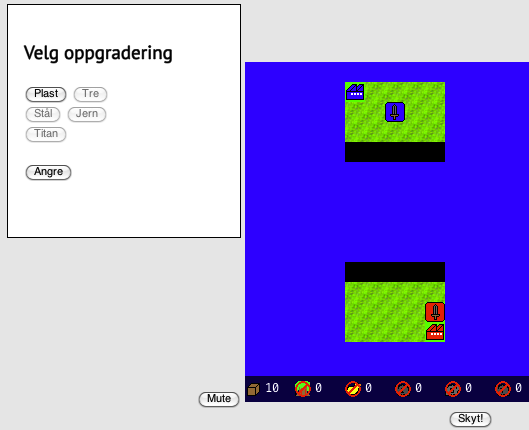
\includegraphics[width=\textwidth]{images/Oppgradering.png}}
\caption{Miljøstasjonen kan oppgraderes til å håndtere ulike typer avfallsgjenvinning.}
\label{fig:Oppgradering}
\end{figure}

\begin{figure}
\centering\setlength\fboxsep{0.2pt}
\setlength\fboxrule{0.7pt}
\fbox{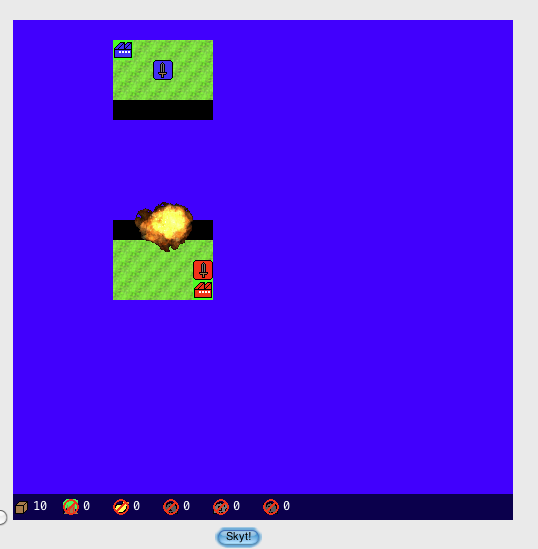
\includegraphics[scale=0.5]{images/Eksplosjon.png}}
\caption{Ved et angrep på en annen spiller vil et projektil avfyres og eksplodere på motspillerens eventuelle forsvarsstruktur.}
\label{fig:Eksplosjon}
\end{figure}

\begin{figure}
\centering
\setlength\fboxsep{0.2pt}
\setlength\fboxrule{0.7pt}
\fbox{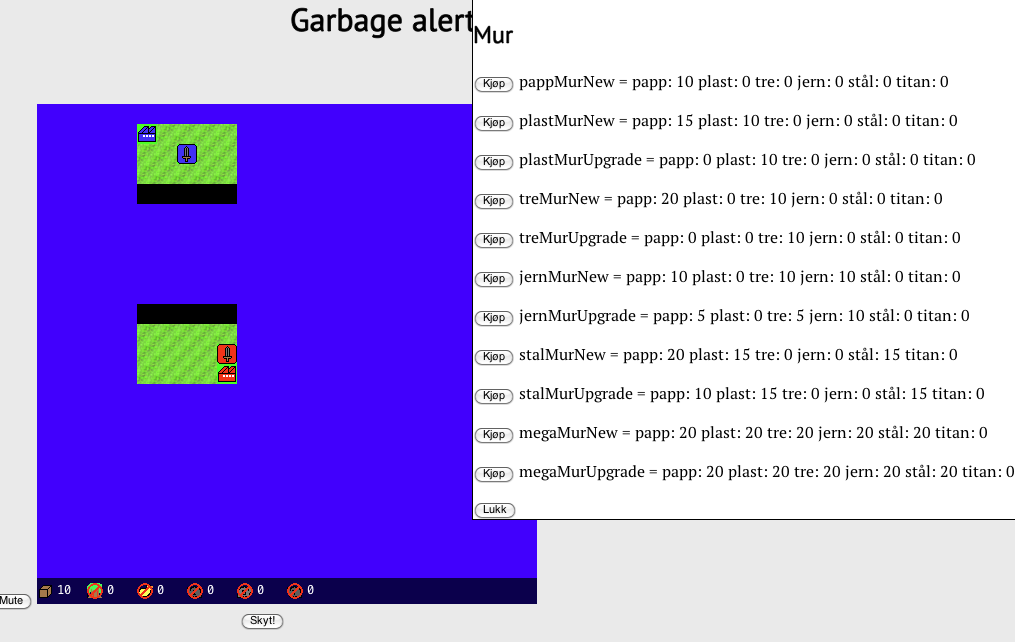
\includegraphics[width=\textwidth]{images/OppgradereMur.png}}
\caption{Spillerens forsvarsstruktur kan oppgraderes til å håndtere sterkere skyts fra motspilleren, avhengig av tilgjengelige ressurser.}
\label{fig:OppgradereMur}
\end{figure}

\begin{figure}
\centering
\setlength\fboxsep{0.2pt}
\setlength\fboxrule{0.7pt}
\fbox{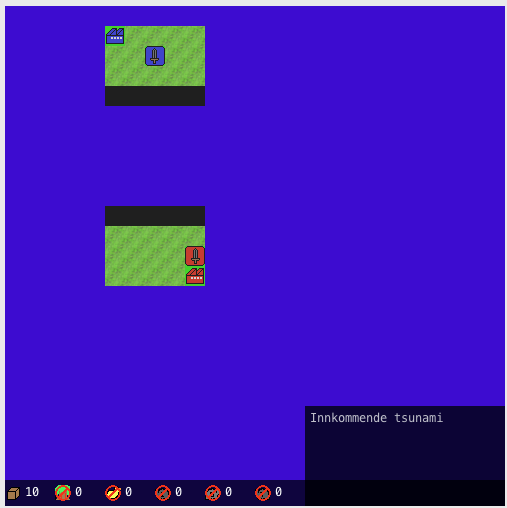
\includegraphics[scale=0.5]{images/Tsunami.png}}
\caption{Globale geohasarder kan oppstå som følge av mye global forsøpling, som for eksempel en tsunami.}
\label{fig:Tsunami}
\end{figure}

\begin{figure} 
\centering
\setlength\fboxsep{0.2pt}
\setlength\fboxrule{0.7pt}
\fbox{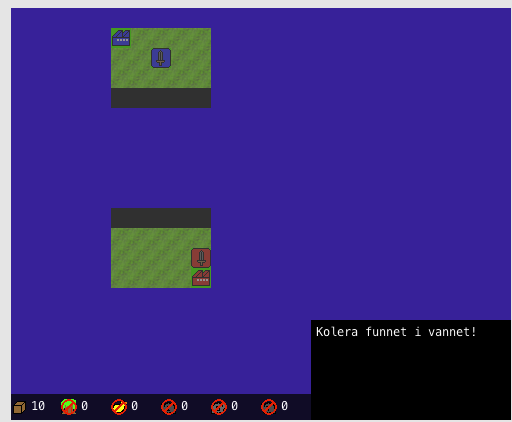
\includegraphics[scale=0.7]{images/Kolera.png}}
\caption{Lokale biohasarder kan oppstå som følge av mye lokal forurensning. Her er et sykdomsutbrudd.}
\label{fig:Kolera}
\end{figure}

\begin{figure} [H]
\centering
\setlength\fboxsep{0.2pt}
\setlength\fboxrule{0.7pt}
\fbox{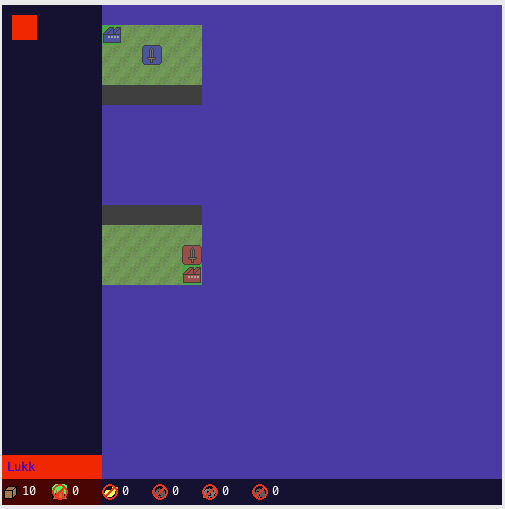
\includegraphics{images/OppgradereEnv.png}}
\caption{Miljøstasjonens effektivitet kan oppgraderes slik at den gjenvinner mer materialer fra hver avfallsenhet.}
\label{fig:OppgradereEnv}
\end{figure}

På figur~\ref{fig:OppgradereEnv} har den røde spilleren åpnet
oppgraderingsmenyen sin. Her har han mulighet til å oppgradere
effektiviteten av miljøstasjonen sin.

Legg merke til at disse skjermskuddene er tatt av en veldig tidlig
prototype som har hatt fokus på å implementere så mye av den tenkte
funksjonaliteten som mulig, heller enn å etablere et konsistent grafisk
uttrykk. Det var ønskelig å benytte så mye som mulig av den kode og
grafikk som ble til i vår tidlige prototype videre i den mer avanserte
prototypen\footnote{Noen vil kanskje si at dette ble gjort i tråd med
landsbyens filosofi om gjenbruk og gjenvinning.}. Mot en sluttfase vil
det være naturlig å erstatte eksempelgrafikken med noe grafikk som er
mer polert.

